\documentclass[12pt, letterpaper]{article}

\usepackage[utf8]{inputenc}
\usepackage[margin=1in]{geometry}
\usepackage{comment}
\usepackage{caption} % for table captions

\usepackage[shortlabels]{enumitem} % for (a) (b) (c) enumerate use [(a)] like so:
%\begin{enumerate}[(a)]
\usepackage{bm}%bold symbols in math mode
\usepackage{amsmath}%allows text in math mode e.g. \text{}

\usepackage{listings} % Typeset Python
%Here is an example of how to do that
%\begin{lstlisting}[language=Python, basicstyle=\tiny]
%#Here is some test Python
%def yay():
%    print("hi")
%\end{lstlisting}

\usepackage{graphicx} % for images
%\includegraphics{uploaded-file-name}

\usepackage{float} % supposedly will allow the use of [H] for table and figure positioning

\title{COSC 5010-03 Practical Machine Learning Fall 2023 Exploratory Data Analysis Report}
\author{Michael Elgin}
\date{November 13, 2023}

\begin{document}

\maketitle

\section{Introduction} %What problem are you solving, how are you going to solve it.

Exploratory data analysis is an important consideration before creating machine-learning models. It can affect the choice of model, the choice of features to prune, or whether samples should be modified or deleted. This report examines the charactersistic of the wine quality dataset\footnote{https://archive.ics.uci.edu/dataset/186/wine+quality}.

\section{Analysis and its Results}

\subsection{Dataset Basics}

The dataset contains 11 features, all of which are real numbers. The quality (target) is an integer. There are a total of 6497 samples. There are no missing values. Approximately 75\% of the samples are white, and 25\% are red.

\subsection{Feature Correlations}

Feature correlations are an important facet of a dataset to explore. The first reason is that there are certain types of models, such as linear models, that expect features not to be correlated. If this is not the case, a linear model may end up assigning unpredictable and inaccurate weights to features. For example, if a linear model predicting circumference of circles is trained on radius as one feature \emph{and} diameter as the second, it may assign an arbitrary weight less than $2\pi$ to the radius and likewise an arbitrary weight less than $\pi$ to the diameter such that the weighted sum always arrives properly at the circumference. But of course in reality this is nonsense; as we know the weights should be \emph{exactly} $2\pi$ and $\pi$ respectively. The issue is correlation, in this case the logical extreme of perfect correlation. Knowing the second value provides no new information and merely creates weights that don't reflect how the feature truly influences the target in reality. The solution is to prune highly correlated features so only one is left.

The second reason is that there is a model-agnostic interpretability method known as partial dependence plots, which are made by creating artificial datasets by setting a feature to be a specific value for all samples, and then finding the model's average prediction for all those samples. Varying the value shows how model prediction changes accordingly (on average). The reason why correlated features are an issue here is that if a plotted feature is correlated with another (unplotted) feature, in reality it won't change by itself. Thus showing how one feature affects model output as it changes independently is misleading because it will never change independently from it's correlated feature. One may observe a change to the feature in the plot and think that the model will also change according to the plot, but it will not because that change in the original feature also involves a hidden change to the correlated feature which will affect model output some way; a way that the partial dependence plot doesn't account for.

Feature correlations are easily visualized by heatmaps. A common technique is to set positively correlated features to one color, negatively correlated features to the opposite color, and no correlations to white. This allows one to easily spot the most correlated features. The correlations for the wine quality dataset are shown in figure \ref{corr}.

\begin{figure}[H]
    \centering
    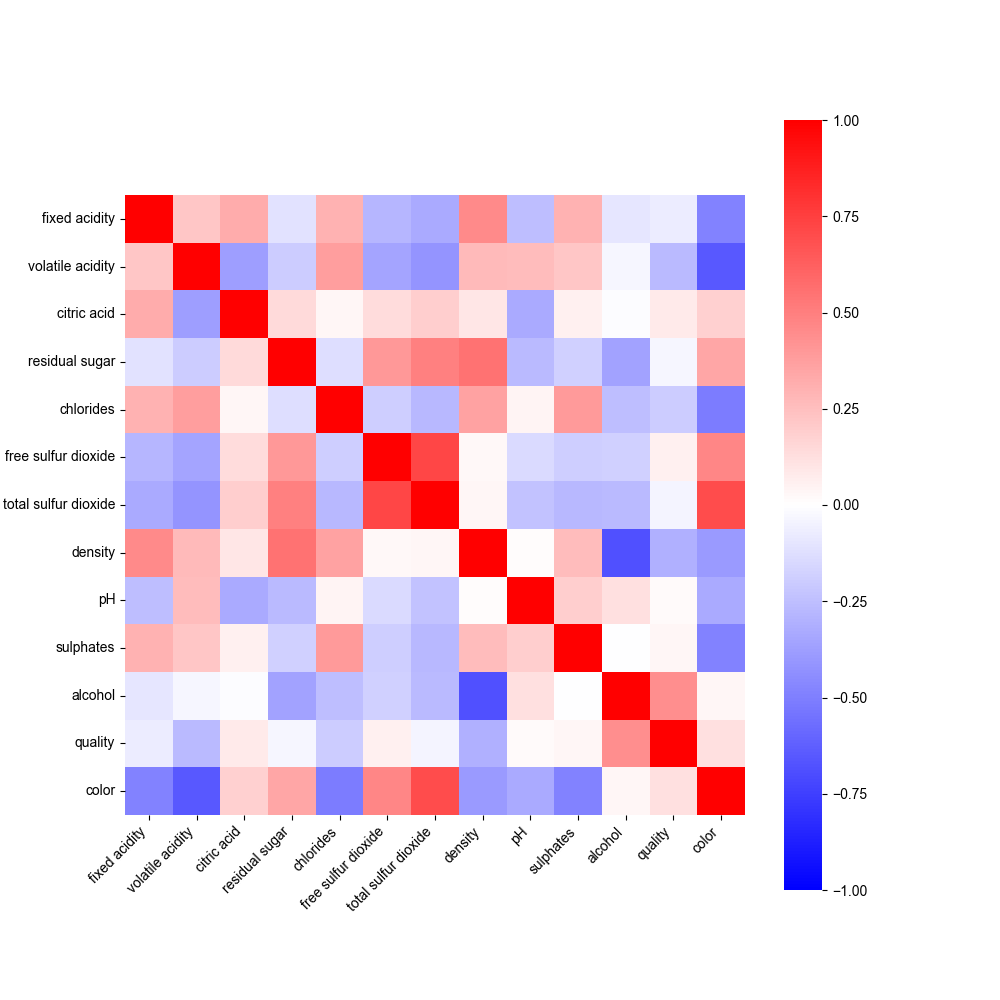
\includegraphics[scale=0.625]{correlations.png}
    \caption{Feature and target correlations}
    \label{corr} % For referencing the figure later in the document
\end{figure}

From here, one can spot free sulphur dioxide and total sulfur dioxide as highly correlated features. This is no surprise, for obvious reasons. At least one of the features should be pruned, most likely total sulfur dioxide. Likewise one can also spot the negative correlation between alcohol and density. This makes intuitive sense, since increasing the amount of alcohol (and thus decreasing water) is always going to change the density in the same direction.

A third reason to know the correlations is to see which features are correlated with the target, as this provides direct insight into which features are influential at changing the target and thus tell something to a model about what target to predict.

\subsection{Class Density Distributions}

An important part of exploratory data analysis involving continuous features and a classification target is to plot the density functions of each class along each feature in the same graph, to see how much separation a feature may give between the classes. This visually shows the differences in features between the classes.

\newcommand{\myscale}{.9775}
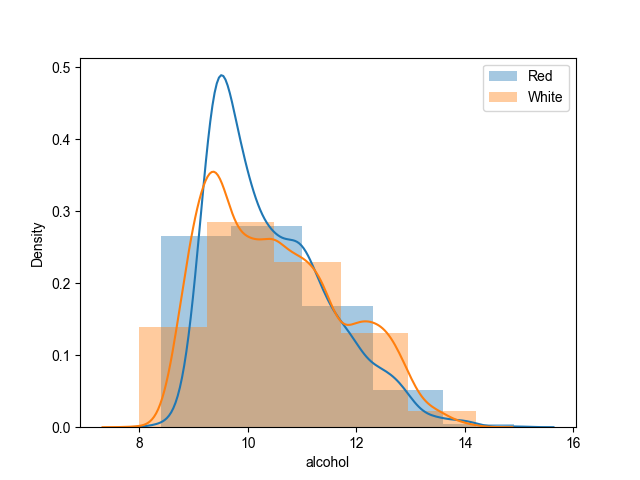
\includegraphics[scale=\myscale]{class_dist_alcohol.png}

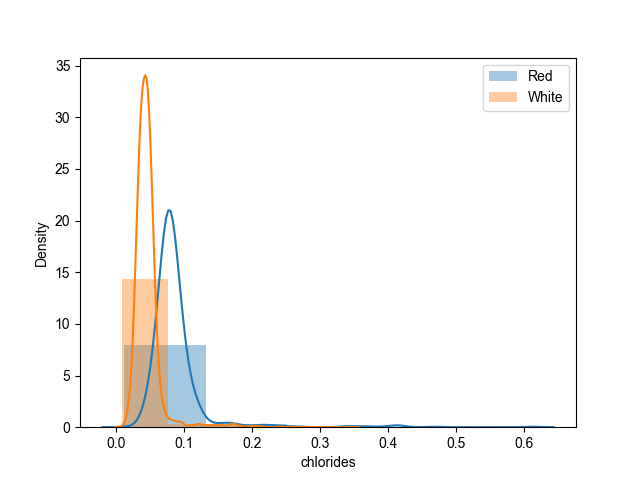
\includegraphics[scale=\myscale]{class_dist_chlorides.png}

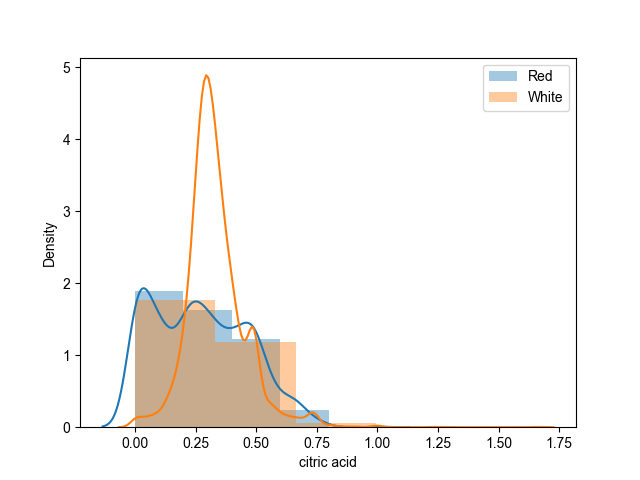
\includegraphics[scale=\myscale]{class_dist_citric_acid.png}

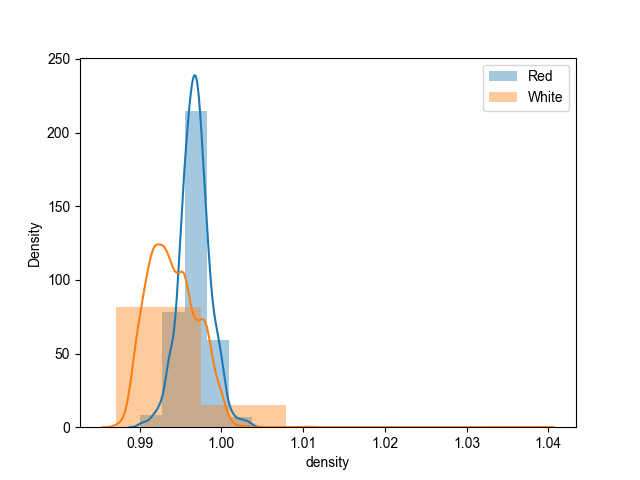
\includegraphics[scale=\myscale]{class_dist_density.png}

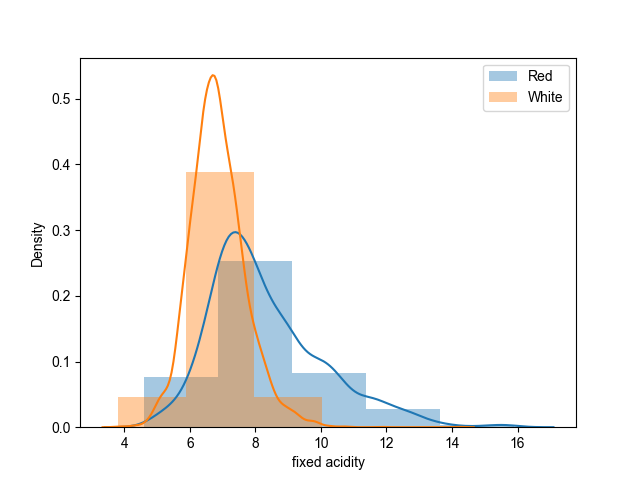
\includegraphics[scale=\myscale]{class_dist_fixed_acidity.png}

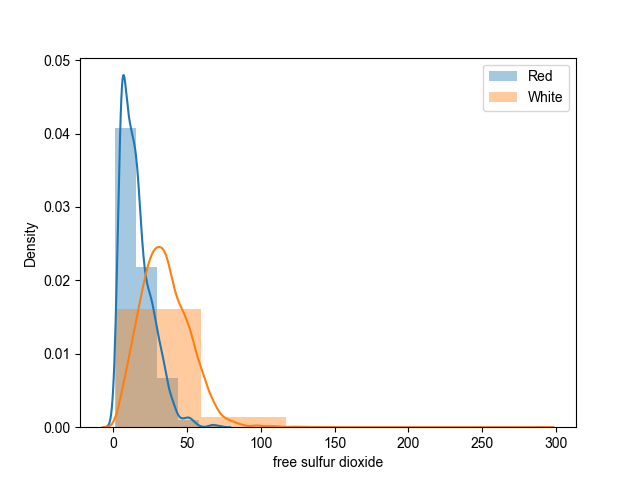
\includegraphics[scale=\myscale]{class_dist_free_sulfur_dioxide.png}

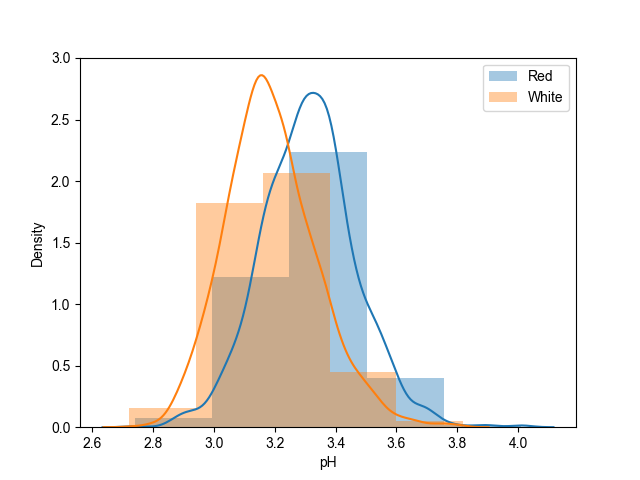
\includegraphics[scale=\myscale]{class_dist_pH.png}

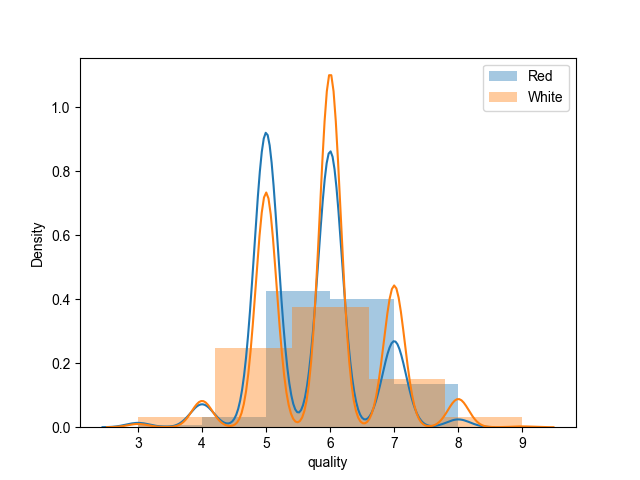
\includegraphics[scale=\myscale]{class_dist_quality.png}

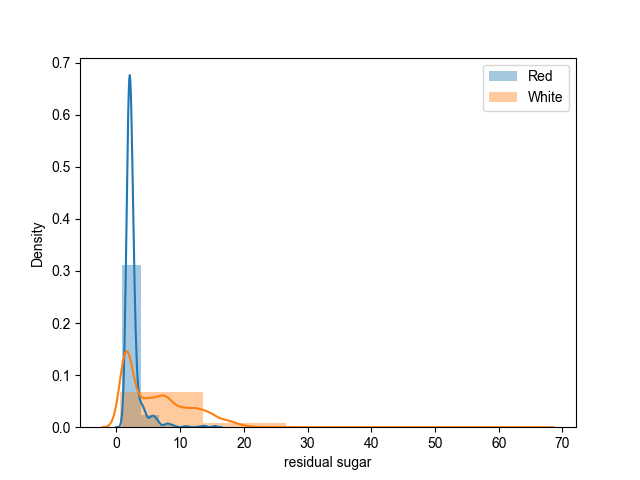
\includegraphics[scale=\myscale]{class_dist_residual_sugar.png}

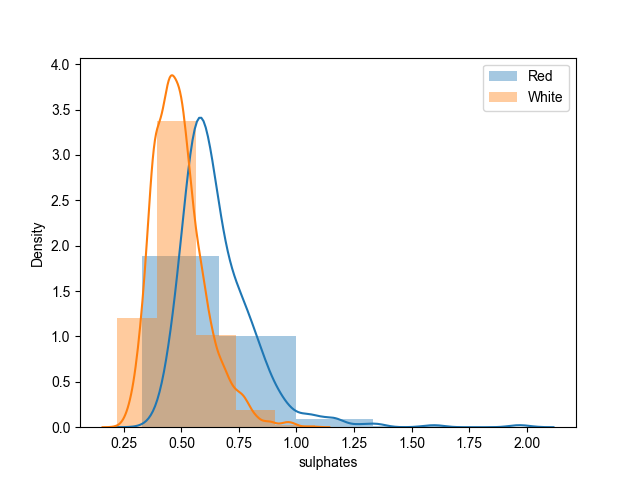
\includegraphics[scale=\myscale]{class_dist_sulphates.png}

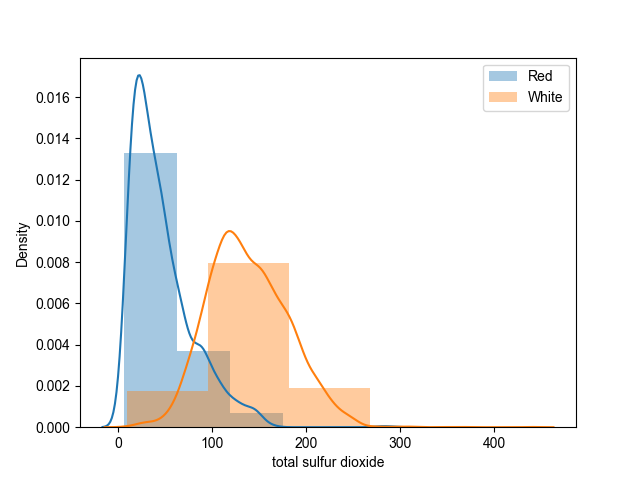
\includegraphics[scale=\myscale]{class_dist_total_sulfur_dioxide.png}

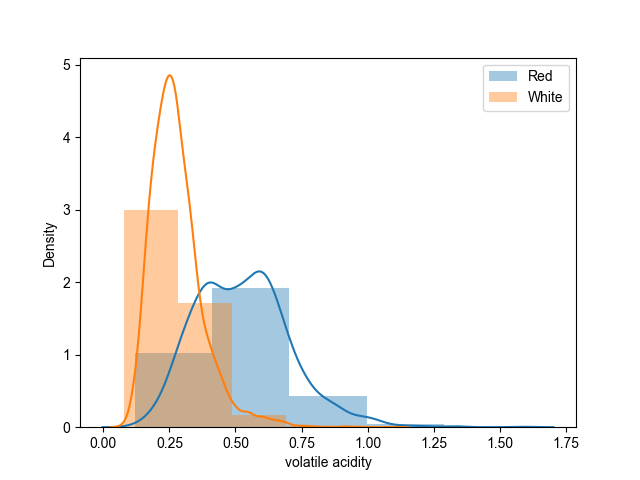
\includegraphics[scale=\myscale]{class_dist_volatile_acidity.png}

There is not complete separation given by any feature. However there is still some healthy separation in chlorides, volatile acidity, free sulfur dioxide, total sulfur dioxide, and residual sugar. These will be features that are likely to be of most use in classification.


\section{Code} %Add the code you've used as a separate file.

The associated code is in EDA.ipynb

\begin{comment} %reference code
    
\section{Dataset Description} %Describe the data you're using, e.g. how many features and observations, what are you predicting, any missing values, etc.

The wine quality dataset is standard tabular data. There are 2 datasets for each color of red and white. Both contain 11 features, all of which are continuous. The target is a discrete value which is the assigned quality of the wine. For the regression tasks, the white wine dataset is used to evaluate models. For classification tasks, both datasets are concatenated, with the target being changed to be the color of the wine, with 0 being assigned to red and 1 to white.

\section{Experimental Setup} %What specifically are you doing to solve the problem, i.e. what programming languages and libraries, how are you processing the data, what machine learning algorithms are you considering, how are you evaluating them, etc.

All computation is done with the Python programming language. Scikit-learn is used to construct models. Pandas is used to load and preprocess the data..

For regression, performance is the mean absolute percentage error, often graphed as its negative (then meaning more is better). This is defined by taking the difference between the predicted value of the model and the actual value, then dividing by the actual value. Then the mean of all of those is taken. More formally:

$$
    GE_{Regression\ model}(\hat{f}, \bm{X}_{test}, \bm{y}_{test}) = \frac{1}{|\bm{X}_{test}|} \sum_{i=1}^{|\bm{X}_{test}|} \frac{\hat{f}(\bm{X}_{test,i} - \bm{y}_{test,i}) \cdot 100}{\bm{X}_{test,i}}
$$

For classification, the performance metric is standard accuracy:

$$
    GE_{Classification\ model}(\hat{f}, \bm{X}_{test}, \bm{y}_{test}) = \frac{\sum_{i=1}^{|\bm{X}_{test}|}l_{0,1}(\hat{f}(\bm{X}_{test,i}), \bm{y}_{test,i})}{|\bm{X}_{test}|}
$$

$$
Acc_{Classification\ model} = (1 - GE_{Classification\ model}) * 100
$$

For all models, grid-search is used for trying hyperparameter configurations. For hyperparameters that are continuous in nature, the grid is exponential in fashion, meaning exponents for $2^x$ are tried. This allows for a much wider exploration of the hyperparameter space given realistic time constraints, since adjusting hyperparameters in a linear fashion would space all configurations too closely together.

Grid search does not use nested resampling. For each hyperparameter config tested, it gathers the score at each cross validation split and as well as the average of those scores. When hyperparameter values are judged here in this report, it is based on the average of the averages of all times they were used. For example, if hypothetical hyperparameter $x = a$ (along with other hyperparameters and their values) is being evaluated, it is cross validated to produce one average, and then the true performance of value $a$ is considered as the average of all the average scores whenever $x$ was $a$ even as other hyperparameter values were different.

The Bayesian optimization by itself does not use nested resampling. It uses a default of 3-fold inner cross-validation. As an additional layer to do nested resampling, 3-fold outer cross-validation wraps this process, and the average of those scores is reported in table \ref{perf_measures}.

The first section is regression models. Model 1 is a decision tree. The hyperparameters considered for this are max depth for the tree and minimum samples required for a split. All hyperparameters explored can only have positive numbers. The minimum amount of samples must be 2, hence the first exponent starts at 1.

$$
\text{max depth} = 2^x, x \in [0,7]
$$

$$
\text{min samples} = 2^x, x \in [1,15]
$$

The second model is a random forest, which uses the same hyperparamters as the tree but also adds in the third hyperparameter of the amount of trees in the forest.

$$
\text{max depth} = 2^x, x \in [0,4]
$$

$$
\text{min samples} = 2^x, x \in [1,4]
$$

$$
\text{number of trees} = 2^x, x \in [0,7]
$$

The second section is classification models. Model 1 is a support vector classifier. Its first hyperparmeter is ``C", which is inverse regularization strength. The second hyperparameter is the kernel type, which is either poly (polynomial) or rbf (radial basis function).

$$
\text{C} = 2^x, x \in [0,15]
$$

$$
\text{kernel type} \in \{\text{poly, rbf}\}
$$

Model 2 is logistic regression, which uses the following hyperparameter settings.

$$
\text{C} = 2^x, x \in [0,8]
$$

$$
\text{penalty type} \in \{\text{l1, l2}\}
$$

Model 3 is a decision tree classifier, which uses the same hyperparmeter settings as in regularization.

$$
\text{max depth} = 2^x, x \in [0,7]
$$

$$
\text{min samples} = 2^x, x \in [1,15]
$$

Model 4 is a K-nearest neighbor classifier, whose hyperparameters are the amount of neighbors to consider and the distance metric.

$$
\text{number of neighbors} = 2^x, x \in [0,7]
$$

$$
\text{distance metric} \in \{\text{l1, l2}\}
$$

Model 5 is a random forest classifier, which uses the same hyperparameters as in regression.

$$
\text{max depth} = 2^x, x \in [0,4]
$$

$$
\text{min samples} = 2^x, x \in [1,4]
$$

$$
\text{number of trees} = 2^x, x \in [0,7]
$$

\section{Results} %Description of what you observed, including plots.

\subsection{Plots of hyperparameter averages}

\newcommand{\myscale}{0.4}

Plots for Decision Tree Regressor hyperparameters:

\includegraphics[scale=\myscale]{decision_tree_regressor_Max Depth.png}

\includegraphics[scale=\myscale]{decision_tree_regressor_Min Samples for Split.png}

Plots for Random Forest Regressor hyperparameters:

\includegraphics[scale=\myscale]{random_forest_regressor_Max Depth.png}

\includegraphics[scale=\myscale]{random_forest_regressor_Min Samples for Split.png}

\includegraphics[scale=\myscale]{random_forest_regressor_Number of Trees.png}

Plots for Support Vector Classifier hyperparameters:

\includegraphics[scale=\myscale]{svc_C Value.png}

\includegraphics[scale=\myscale]{svc_Kernel Type.png}

Plots for Logistic Regression hyperparameters:

\includegraphics[scale=\myscale]{logistic_regression_C Value.png}

\includegraphics[scale=\myscale]{logistic_regression_Penalty Type.png}

Plots for K-Nearest Neighbor hyperparameters:

\includegraphics[scale=\myscale]{knn_Number of Neighbors.png}

\includegraphics[scale=\myscale]{knn_Metric.png}

Plots for Decision Tree Classifier:

\includegraphics[scale=\myscale]{decision_tree_classifier_Max Depth.png}

\includegraphics[scale=\myscale]{decision_tree_classifier_Min Samples for Split.png}

Plots for Random Forest Classifier:

\includegraphics[scale=\myscale]{random_forest_classifier_Max Depth.png}

\includegraphics[scale=\myscale]{random_forest_classifier_Min Samples for Split.png}

\includegraphics[scale=\myscale]{random_forest_classifier_Number of Trees.png}

Combination plots follow\footnote{
Note that the time cost of grid-search kept more values from being explored.
}.

\includegraphics[scale=\myscale]{combo_C.png}

\includegraphics[scale=\myscale]{combo_max_depth.png}

\includegraphics[scale=\myscale]{combo_min_samples_split.png}

\includegraphics[scale=\myscale]{combo_n_estimators.png}

For some hyperparameters, similar trajectories were observed between models. For others there was no reliable pattern across the space of values.

\subsection{Tables of best hyperparameters}

The following tables show the best configurations found from grid-search. These do not always match the best points on the plots of the averages because occasionally the combination of several hyperparameter settings that weren't optimal on average can still be the best when working together. The first value is from grid-search, the second is from Bayesian optimization. Note that results from runs of Bayesian optimization may vary if the random\_state seed is changed from 0.

\begin{table}[H]
\centering
\caption{Regression models' best hyperparameters}
\label{reg_table}
\begin{tabular}{c|c|c|c} % l for left-aligned column, c for centered columns
                & Max Depth     & Min Samples for Split & Number of Trees \\ \hline
Decision Tree   & 8, 44            & 512, 582                  &   \\
Random Forest   & 8, 8             & 8, 8                    & 64, 58 \\
\end{tabular}
\end{table}

\begin{table}[H]
\centering
\caption{Classification models' best hyperparameters}
\label{cls_table 1}
\begin{tabular}{c|c|c|c} % l for left-aligned column, c for centered columns
                            & C         & Kernel Type   & Penalty Type \\ \hline
Support Vector Classifier   & 16348, 15846     & rbf, rbf \\
Logistic Regression         & 64, 81        &               & l2, l2 \\
\end{tabular}
\end{table}

\begin{table}[H]
\centering
\caption{Classification models' best hyperparameters}
\label{cls_table 2}
\begin{tabular}{c|c|c|c} % l for left-aligned column, c for centered columns
                & Number of Neighbors & Distance Metric\\ \hline
K-Nearest Neighbor & 8, 10 & l1, l1 \\
\end{tabular}
\end{table}

\begin{table}[H]
\centering
\caption{Classification models' best hyperparameters}
\label{cls_table 3}
\begin{tabular}{c|c|c|c} % l for left-aligned column, c for centered columns
                & Max Depth     & Min Samples for Split     & Number of Trees \\ \hline
Decision Tree   & 32, 58 & 2, 2 \\
Random Forest   & 8, 8 & 2, 8 & 32, 54 \\
\end{tabular}
\end{table}

\subsection{Table of performance measures for grid-search and Bayesian optimization}

\begin{table}[H]
\centering
\caption{Performance comparison for grid-search and Bayesian optimization}
\label{perf_measures}
\begin{tabular}{c|c|c} % l for left-aligned column, c for centered columns
                            & Grid Search     & Bayesian Optimization  \\ \hline
Decision Tree Regressor     & -0.1070 & -0.1035 \\
Random Forest Regressor     & -0.1014 & -0.0946\\
Support Vector Classifier   & 98.815\% & 98.876\%\\
Logistic Regression         & 98.815\% & 98.784\%\\
K-Nearest Neighbors         & 94.582\% & 94.875\%\\
Decision Tree Classifier    & 98.107\% & 98.306\%\\
Random Forest Classifier    & 99.338\% & 99.369\%\\
\end{tabular}
\end{table}

Based on the table, it is not clear whether grid-search or Bayesian optimization is ``better" than the other. There were some cases where each produced a final model that had slightly better performance than the other. In all cases, the differences were trivial.

\end{comment}

\end{document}